\subsection{Summary of Work}
The objective of this work is to identify the existence probability of a semi-orthogonal user selection group as a function of SNR and SIR requirements, group size, number of transmit antennas, and the number of users or stations (STAs) considered as candidates for addition to the semi-orthogonal user selection group. 

The rate of growing the number of users considered vs. increasing the SNR requirements is also investigated asymptotically.

\subsection{SNR ad SIR Requirements}
The requirement for a $\epsilon$-orthogonal group (semi-orthogonal user selection group, or SUS group) is broken into two parts. Firstly the users in the group are required to have a channel norm similar to other users in the group. The upper and lower bound on SNR ensures that users in an SUS group have similar channel gains. Asserting an upper and lower bound can be viewed a coarse form of power control. The upper and lower bound can be adjusted to a narrow improving linear precoding or fine power control performance. Since the norms of the channels in the SUS group are similar, the precoding weights should also be similar, allowing for more even distribution of weights between precoding factors.

The second requirement deals with interference between users in an SUS group. Once it has been determined that a given user meets the SNR requirement, then it is compared against other candidate users to ensure interference is sufficiently low. The inner product between a user's channel and other candidate user's channels is formed. The magnitude of the product is compared to some threshold , $\epsilon$. If the product is lower than the threshold, users are said to be $\epsilon$-orthogonal and the users are added to the SUS group.

The expression for a SUS group requirements is given by as:

\begin{equation}\label{eq:S_e}
    \begin{aligned}
        \mathcal{S}_\epsilon = \lbrace \mathcal{S}_a \big|\ | \textbf{h}_i\textbf{h}_j^H |\ <\ \epsilon \ \text{;} \ \rho^-<\Vert \textbf{h}_i \Vert^2 < \rho^+\ \forall \ i \neq j \in \mathcal{S}_a \rbrace
    \end{aligned}
\end{equation}

\subsection{Existence Probability of SUS Groups}
The main contribution of the work is to develop an expression for the existence probability of an SUS group. Swannack develops a lower bound on the existence probability, $Pr[\mathcal{S}_\epsilon \neq \lbrace \emptyset \rbrace]$. Probability of SUS group existence depends on the orthogonality requirements given in Eq. (\ref{eq:S_e}), the group size $l = \vert \mathcal{S}_a \vert$, and the number of candidate users considered for addition to the SUS group, $n$. 

Swannack considers an example to illustrate results. The example is shown in Fig. \ref{fig:swannack_fig5a}, this example was replicated with results of replication shown in Fig. \ref{fig:reproduce_fig5a}. The purpose of this example is to determine the number of users that must be evaluated for addition to an SUS group of size 2, 3, and 4 to achieve a probability of existence of 90\%. In this example 4 transmit antennas are assumed.

\begin{figure}
    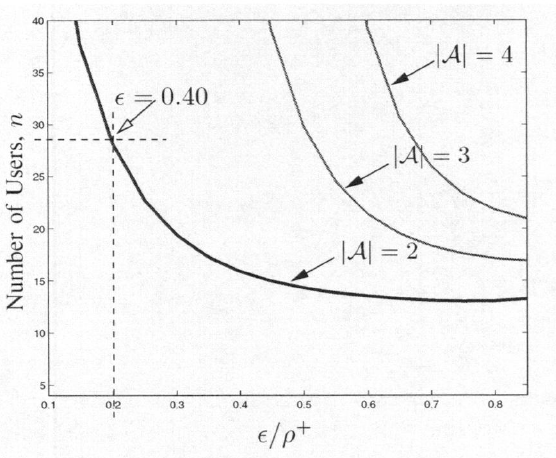
\includegraphics[width=12cm]{figs/swannack_fig5a.png}\\
    \caption{Plot of minimum number of users to achieve minimum probability of SUS group existence of 0.9. 4 transmit antennas are assumed for all curves.}
    \label{fig:swannack_fig5a}
\end{figure}

\begin{figure}
    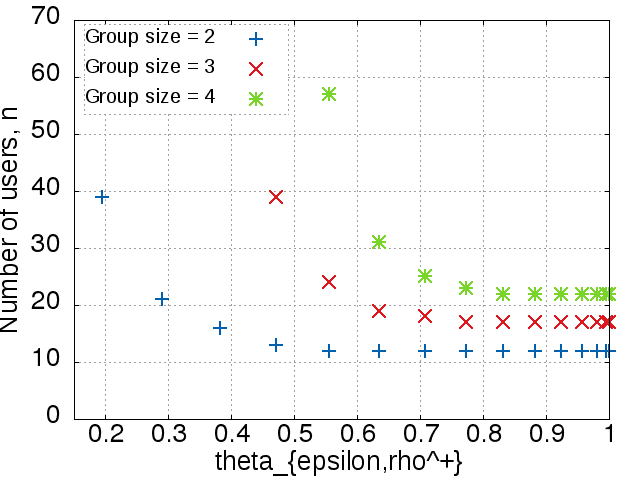
\includegraphics[width=12cm]{figs/existence.png}\\
    \caption{Plot of minimum number of users to achieve minimum probability of SUS group existence of 0.9. 4 transmit antennas are assumed for all curves. Horizontal axis scale is $\cos{(\theta_\epsilon,\rho^+)} = \frac{\epsilon}{\rho^+}$}
    \label{fig:reproduce_fig5a}
\end{figure}

The results shown in Fig. \ref{fig:swannack_fig5a} are developed a geometric interpretation. The geometric interpretation developed by Swannack involves projecting channel onto the surface of complex $m$-dimensional sphere (where $m$ is analogous to the number of transmit antennas), then considering probability of overlapping spherical caps in this space. The gometric model is split into two parts: the SNR requirement, and this SIR (orthogonality) requirement.

The geometric analog of user $i$'s channel, $\textbf{h}_i$, satisfying the SNR requirement is that $\Vert\textbf{h}_i\Vert^2$ lies in the real spherical 2$m$ shell between $\rho^-$ and $\rho^+$. The geometric analog of the orthogonality requirement is that the angle formed between any two channels in the SUS group are greater than $\arccos{(\frac{\epsilon}{\rho^+})}$. First we consider SNR requirement developed by Swannack.

It is assumed that $\textbf{h}_i$ is a circularly symmetric Gaussian random variable with zero mean and variance  $\frac{1}{2m}$. Therefore the L2 norm of the channel will follow a Gamma distribution, since the L2 norm is essentially a sum of squared normally distributed random variables with zero mean constant variance $\neq 1$. It is also assumed that the SUS group size is equal to the number of transmit antennas, m: $\vert \mathcal{S}_a\vert = m$. Note that the incomplete gamma function in (\ref{eq:p_s}) are assumed to be normalized. A more detailed discussion of manipulation of normal distributions, associated Gamma distributions is provided in the appendices. 

 We can apply Eq. (\ref{eq:gamma_scaled}) from the appendix in order to develop an expression for the CDF of the channel norm. The CDF of the channel norm will be denoted by $F_{\Vert\textbf{hi}\Vert^2}(m,\rho)$, where $\rho$ are realizations of the random variable formed by the channel norm. 

Each term in the $m$-length vector, $\textbf{h}_i$ is represented by two normal random variables: one for the real part and one for the imaginary part. When forming the L2 norm of the $m$-length vector, each multiplication forms a sum of length four where each of the arguments of the sum are a product of two random variables. Namely, the sum takes the form real$\cdot$real + real$\cdot$imaginary + imaginary$\cdot$real + complex$\cdot$complex. Even though this sum can be simplified to a complex number, each term in the sum adds a degree of freedom to the resulting Gamma distribution. Thus, when forming the CDF , the expression becomes:

\begin{equation}\label{eq:ch_sq_cdf_chan}
    \begin{aligned}
        F_{\Vert\textbf{hi}\Vert^2}(\rho;m)& = \Gamma_n(2m,m\rho)\\
        &= Pr[\Vert\textbf{h}_i\Vert^2 \leq \rho]
    \end{aligned}
\end{equation}

Thus, in the complex-channel case presented by Swannack, the probability that the channel satisfies SNR requirements, namely that $\Vert\textbf{h}i\Vert^2$ lands in the shell between radii $\rho^+,\ \rho^-$,  is given by the subtraction of the respective CDF expressions:
\begin{equation}\label{eq:p_s}
    \begin{aligned}
        p_s = \Gamma_n(2m,m\rho^-) - \Gamma_n(2m,m\rho^+)
    \end{aligned}
\end{equation}

Now we turn our attention to Swannack's expression of the conditional probability that the orthogonality requirement is met, given that the channel norm falls between $\rho^-$ and $\rho^+$. The conditional probability is defined as $p_\perp$. Swannack develops a lower bound on the probability associated with the orthogonality constraint, $p_\perp$, as:
\begin{equation}\label{eq:p_perp}
    \begin{aligned}
        p_\perp \geq (1-(1-l)\delta_c(\theta_{\epsilon,\rho},2m))^{l-1}
    \end{aligned}
\end{equation}

The function $\delta_c(\theta,2m)$ is defined as the ratio of the area of a spherical (polar) caps of a sphere in $2m$ dimensions formed by $\theta$ to the entire surface area of the sphere:

\begin{equation}\label{eq:delta_c_sphere}
    \begin{aligned}
        \delta_c(\theta,2m) = 2\frac{\Omega_{2m}(\theta)}{\Omega_{2m}(\pi)}
    \end{aligned}
\end{equation}

Swannack develops upper and lower bounds on $\delta_c$ (TODO: elaborate on these bounds as necessary--will likely be required as we consider developing new bounds in the widely linear case).

Some investigation into the impact of change in number of dimensions on $\delta_c$ lower bounds are shown in Fig. \ref{fig:delta}.
\begin{figure}
    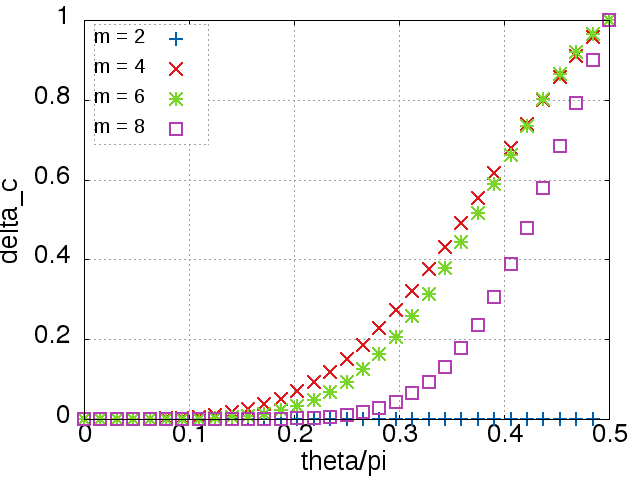
\includegraphics[width=12cm]{figs/delta.png}\\
    \caption{Plot of $\delta_c$ as a function of $\theta_{\epsilon,\rho}$ over various dimensions (ie. number of transmit antennas)}
    \label{fig:delta}
\end{figure}

Several additional plots investigating impact of changes in SUS group size and number of dimensions are shown in Figs. \ref{fig:p_orth_gs_2}, \ref{fig:p_orth_gs_4}, \ref{fig:p_orth_gs_6}, \ref{fig:p_orth_gs_8}.

\begin{figure}
    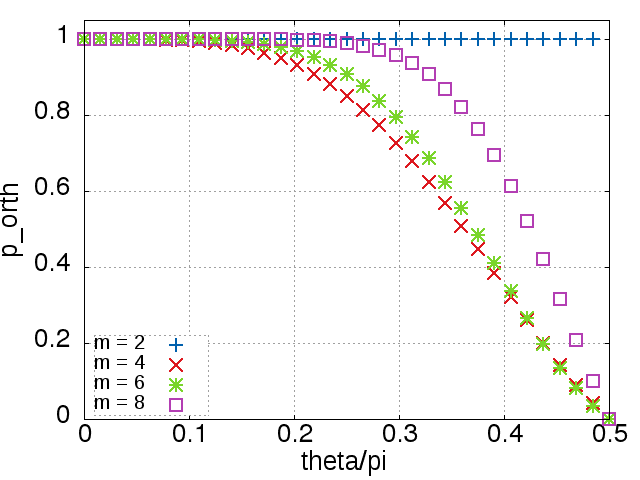
\includegraphics[width=12cm]{figs/p_orth_gs_2.png}\\
    \caption{Plot of $p_{\perp}$ as a function of $\theta_{\epsilon,\rho}$ over various dimensions (ie. number of transmit antennas), SUS group size of 2}
    \label{fig:p_orth_gs_2}
\end{figure}

\begin{figure}
    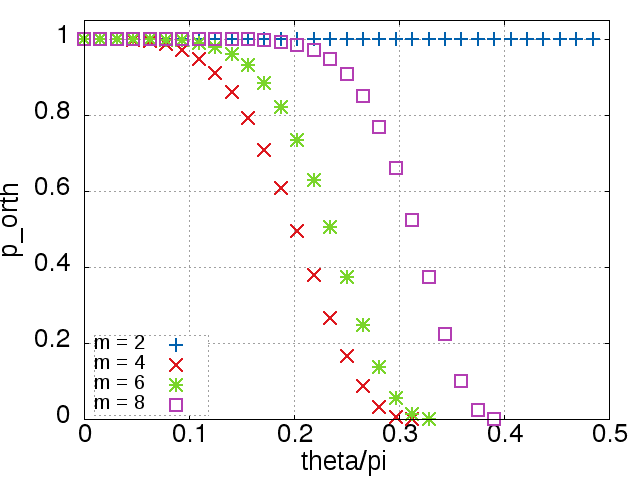
\includegraphics[width=12cm]{figs/p_orth_gs_4.png}\\
    \caption{Plot of $p{\perp}$ as a function of $\theta_{\epsilon,\rho}$ over various dimensions (ie. number of transmit antennas), SUS group size of 4}
    \label{fig:p_orth_gs_4}
\end{figure}

\begin{figure}
    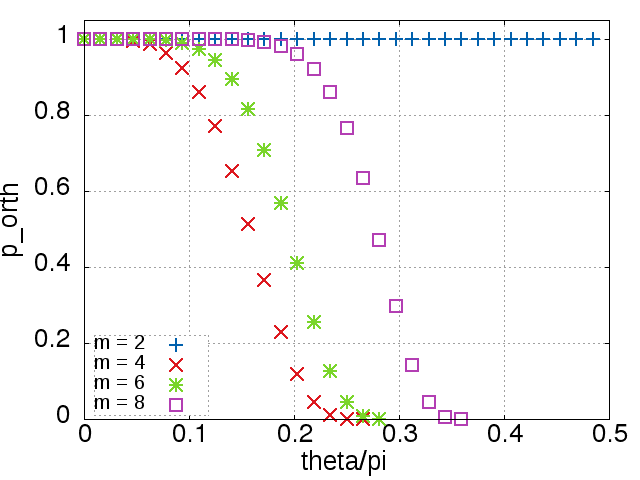
\includegraphics[width=12cm]{figs/p_orth_gs_6.png}\\
    \caption{Plot of $p{\perp}$ as a function of $\theta_{\epsilon,\rho}$ over various dimensions (ie. number of transmit antennas), SUS group size of 6}
    \label{fig:p_orth_gs_6}
\end{figure}

\begin{figure}
    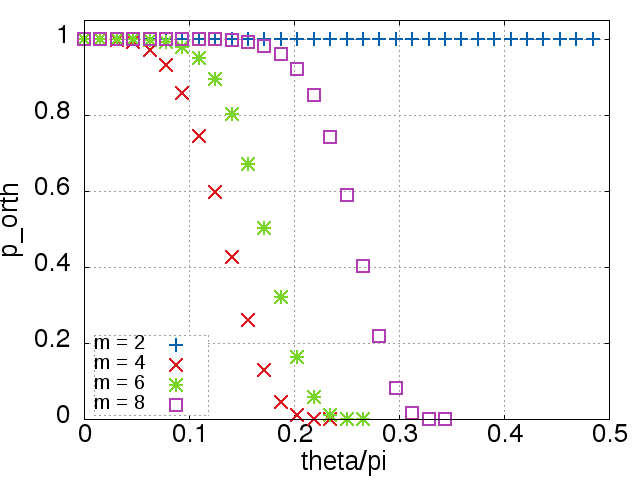
\includegraphics[width=12cm]{figs/p_orth_gs_8.png}\\
    \caption{Plot of $p{\perp}$ as a function of $\theta_{\epsilon,\rho}$ over various dimensions (ie. number of transmit antennas), SUS group size of 8}
    \label{fig:p_orth_gs_8}
\end{figure}
%%%%%%%%%%%%%%%%%%%%%%%%%%%%%%%%%%%%%%%%%%%%%%%%%%%%%%%%%%%%%%%%%%%%%%%%%%%%%%%%%%%%%%%%%%%%%%%%%%%%%%%%%%%%%%%%%%%%%%
\newpage
\subsection{Extending results to incorporate path loss}
%%%%%%%%%%%%%%%%%%%%%%%%%%%%%%%%%%%%%%%%%%%%%%%%%%%%%%%%%%%%%%%%%%%%%%%%%%%%%%%%%%%%%%%%%%%%%%%%%%%%%%%%%%%%%%%%%%%%%%
In this section we set out to incorporate a path loss model into Swannack's results. An exponential path loss model is assumed. The distribution of users (or STAs) is assumed to follow a two-dimensional Poisson point process(PPP); therefore the path loss is stochastic in nature. The incorporation of a path loss model impacts the expression for $p_s$ given in Eq. (\ref{eq:p_s}); however, it does not impact $p_\perp$ since this probability is conditioned on the channel norm falling into the shell between radii $\rho^-,\rho^+$.

When we incorporate path loss, the channel vector, $\textbf{h}_i$ is no longer composed of standard normal random variables. Rather, each of the random variables is scaled by a path loss factor. Therefore, the channel becomes:
\begin{equation}\label{eq:pl_channel}
    \begin{aligned}
        \Tilde{\bold{h}_i} &= \sqrt{\alpha_i}\textbf{h}_i \sim\mathcal{N}(0,\frac{\alpha_i)}{2m};\\
        \alpha_i &= d_i^{-\eta};\\
        d_i &\in \Phi_{2D} \sim P[N(A)=k;\lambda] = \frac{k^{\lambda A}}{k!}e^{-\lambda A}
    \end{aligned}
\end{equation}
The distance for the $i^{th}$ STA,$d_i$, follows a PPP, as previously mentioned. Therefore, the variance of the normal distribution becomes stochastic. This implies that the parameters of the resulting Gamma distribution, representing the channel norm, will also be stochastic. The CDF expression incorporating path loss, which may be compared to Eq. (\ref{eq:ch_sq_cdf_chan}), is given by:
\begin{equation}\label{eq:ch_sq_cdf_chan_pl}
    \begin{aligned}
        F_{\Vert\Tilde{\bold{h}i}\Vert^2}(\rho;m,\alpha_i)& = \Gamma_n(2m,m\rho/\alpha_i)\\
        &= Pr[\Vert\Tilde{\bold{h}_i}\Vert^2 \leq \rho]
    \end{aligned}
\end{equation}
Although the expressions in Eqs. (\ref{eq:ch_sq_cdf_chan}),(\ref{eq:ch_sq_cdf_chan_pl}), appear similar at first glance, the stochastic parameter $\alpha_i$ in Eq. (\ref{eq:ch_sq_cdf_chan_pl}) must be translated into a scalar quantity for the expressions to be comparable.

Such a translation may be formulated as an estimation problem. For example, a minimum mean squared estimation of $\alpha_i$, $\Hat{\alpha_i}$, may be calculated, then $\Hat{\alpha_i}$ may be used in order to find the probability associated with the CDF in Eq. (\ref{eq:ch_sq_cdf_chan_pl}).

This approach has several challenges. Firstly, we must find an expression for the PDF for $\alpha_i$. This PDF, $f_{\alpha i}(\alpha_i;\lambda,\eta)$, is denoted by $\omega(\alpha_i)$ in the context of the estimation discussion. It does not make physical sense to simply apply a transformation to the PPP PMF without considering what the PMF physically represents; applying the exponential transformation directly to the PPP PMF does not result in anything physically sensical or useful. Therefore, we now devise a more physically reasonable approach.

We begin by defining a circle, $C_{di}$, of radius $d_i$ that is centred at the AP. The user $i$ lies on the circle $C_{di}$. Next we define two more circles concentric to $C_{di}$, $C_{di+\Delta}$ and $C_{di-\Delta}$. The radius of $C_{di+\Delta}$ and $C_{di\Delta}$ is $d_i + \Delta$ and $d_i - \Delta$, respectively. Relating these circles back to a physical context we can make several observations. Firstly, since user $i$ lies on the circle $C_{di}$, its path loss will be $\alpha_i = d_i^{-\eta}$.  Secondly, the probability that $k$ STAs lie between the area falling between circles $C_{di-\Delta}$ and $C_{di+\Delta}$ will follow the PMF:
\begin{equation}\label{eq:ppp_pmf_circle}
    \begin{aligned}
        \Phi_{di\pm\Delta} \sim P[N(A_{di\pm\Delta})=k;\lambda] = \frac{(\lambda A_{di\pm\Delta})^k}{k!}e^{-\lambda A_{di\pm\Delta}}
    \end{aligned}
\end{equation}
where $A_{di\pm\Delta}$ is the doughnut-shaped area formed between $C_{di-\Delta}$ and $C_{di+\Delta}$. Thirdly, we note that the homogeneous PPP of STAs is rotation-invariant about the centre of the concentric circles, and invariant on radial translation with respect to the centre of the circles. Therefore, $A_{di\pm\Delta}$ is given by:
\begin{equation}\label{eq:disk_area}
    \begin{aligned}
        A_{di\pm\Delta} &= 2\pi\int_{di-\Delta}^{di+\Delta}r\ dr\\
        &= 4d_i\Delta
    \end{aligned}
\end{equation}
Notice that as $\Delta \rightarrow 0$, $P[N(A_{di\pm\Delta})=k;\lambda] \rightarrow 0$ as well. However, as $\Delta \rightarrow 0$, the STAs contained in the $A_{di\pm\Delta}$ will have more similar path loss values. If we approximate all the STAs in $\in\ A_{di\pm\Delta}$, to have a path loss of $\alpha_i$, this behaviour becomes a tradeoff between accuracy of the model and probability that another STA will exist in $A_{di\pm\Delta}$.

Such an accuracy-existence tradeoff should be able to be linked back to the original SNR requirement in terms of $\rho^+,\rho^-$ and SUS group existence probability. However, if we crudely ignore the impact truncating STA path loss, the original expression for $p_s$ given in Eq. (\ref{eq:p_s}) remains the same. The bounds of $\rho^-,\rho^+$ will differ from the original values given by Swannack on a case-by-case basis since channel norms will now be attenuated by path loss (ie. original $\rho$ values should also be scalsed by path loss). The expression for existence probability of an SUS group is expected to be impacted by the factors associated with the PPP, namely the value of $\Delta$.
%%%%%%%%%%%%%%%%%%%%%%%%%%%%%%%%%%%%%%%%%%d%%%%%%%%%%%%%%%%%%%%%%%%%%%%%%%%%%%%%%%%%%%%%%%%%%%%%%%%%%%%%%%%%%%%%%%%%%%%
\newpage
\subsection{Extending results to relaxed orthogonality constraint}
%%%%%%%%%%%%%%%%%%%%%%%%%%%%%%%%%%%%%%%%%%%%%%%%%%%%%%%%%%%%%%%%%%%%%%%%%%%%%%%%%%%%%%%%%%%%%%%%%%%%%%%%%%%%%%%%%%%%%%
We now consider relaxing the orthogonality and SNR constraints, by limiting  requirements to only the real part of the channel inner product and norm. First we introduce the following definitions. Let the  transformation, $\mathcal{T}$, be the transformation of the complex vector in $\mathbb{C}^m$ to a real vector in $\mathbb{R}^{2m}$:
\begin{equation}\label{eq:complex_real_xform}
    \begin{aligned}
        \textbf{h}_i \in \mathbb{C}^m \xrightarrow{\mathcal{T}} \overline{\textbf{h}}_i = [ \mathfrak{Re} \lbrace \textbf{h}_i \rbrace \ \mathfrak{Im}\lbrace \textbf{h}_i \rbrace ] \in \mathbb{R}^{2m}
    \end{aligned}
\end{equation}
Thus,
\begin{equation}\label{eq:orth_real_transp}
    \begin{aligned}
        \mathfrak{Re} \lbrace \textbf{h}_i\textbf{h}_j^H \rbrace = \overline{\textbf{h}}_i \overline{\textbf{h}}_j^T 
    \end{aligned}
\end{equation}

Following from these definitions and Swannack's expression for SUS groups meeting SNR and orthogonality requirements, the relaxed expression for the collection of SUS groups becomes:
\begin{equation}\label{eq:wl_S_e}
    \begin{aligned}
        \mathcal{S}_{\epsilon,\mathfrak{R}} = \lbrace \mathcal{S}_a \big|\  \overline{\textbf{h}}_i \overline{\textbf{h}}_j^T<\ \epsilon_{\mathfrak{R}} \ \text{;} \ \rho^-<\Vert \overline{\textbf{h}}_i \Vert^2 < \rho^+\ \forall \ i \neq j \in \mathcal{S}_a \rbrace
    \end{aligned}
\end{equation}

The geometric model developed by Swannack is still useful in the relaxed widely linear case given in (\ref{eq:wl_S_e}). However, further discussion regarding expressions for relaxed $p_s$, $p_\perp$ is required. SNR requirements, associated with $p_s$ will be discussed first, then SIR requirements, associated with $p_\perp$ will be discussed.

For the relaxed SNR requirement,the Gamma distribution used to derive the expression in (\ref{eq:p_s}), now only has 2$m$ degrees of freedom, rather than 4$m$ degrees of freedom since the inner product form a sum of 2$m$ real components. Therefore the expression for relaxed probability the norm will fall in the shell defined by radii $\rho^-,\rho^+$, $p_{s,\mathfrak{R}}$ becomes:
\begin{equation}\label{eq:p_s_real}
    \begin{aligned}
        p_{s,\mathfrak{R}} = \Gamma_n(m,m\rho^-) - \Gamma_n(m,m\rho^+)
    \end{aligned}
\end{equation}

Turning our attention now to the SIR requirements, we must now compare the expressions $\overline{\textbf{h}}_i \overline{\textbf{h}}_j^T < \epsilon_\mathfrak{R}$ and $\vert \textbf{h}_i\textbf{h}_j^H \vert < \epsilon$. Specifically, we set out to determine the relationship between $\epsilon$ and $\epsilon_\mathfrak{R}$ such that the two inner products are comparable or equivalent.

One such approach is to view the relaxed inner product that lives in $\mathbb{R}^{2m}$ as a widely linear transformation of the original complex expression that lives in $\mathbb{C}^{m}$. As shown in \cite{Adali2011}, the inner products can be related as follows:
\begin{equation}\label{eq:wl_inner_product}
    \begin{aligned}
       \overline{\textbf{h}}_i \overline{\textbf{h}}_j^T = \frac{1}{2}\vert \textbf{h}_i\textbf{h}_j^H \vert
    \end{aligned}
\end{equation}
A proof of this expression is offered in the Appendices.
%%%%%%%%%%%%%%%%%%%%%%%%%%%%%%%%%%%%%%%%%%%%%%%%%%%%%%%%%%%%%%%%%%%%%%%%%%%%%%%%%%%%%%%%%%%%%%%%%%%%%%%%%%%%%%%%%%%%%%